\documentclass[sigconf]{acmart}
\usepackage{graphicx}
\usepackage{float}
\usepackage{amsmath}
\begin{document}
\title{Secure Digital Signature Validated by Ambient}
\author{User's Wi-Fi-enabled devices}
\affiliation{\institution{North Carolina A&T State University}}
\email{AlQahtani.aasa@gmail.com}
\author{Ali Abdullah S. AlQahtani}
\affiliation{\institution{Computer science}}
\email{hosam.amleh@gmail.com}
\author{Computer Systems Technology}
\affiliation{\institution{University of North Carolina Wilmington}}
\email{Znelawadi@gmail.com}
\author{Greensboro}
\affiliation{\institution{Cyberspace Engineering}}
\author{North Carolina}
\affiliation{\institution{Louisiana Tech University}}
\author{USA}
\author{Hosam Alamleh}
\author{Wilmington}
\author{NC}
\author{Zakaria El-Awadi}
\author{Ruston}
\author{Louisiana}
\author{USA}
\begin{abstract}
In cyberspace, a digital signature is a mathematical technique that plays a significant role, especially in validating the authenticity of digital messages, emails, or documents. Furthermore, the digital signature mechanism allows the recipient to trust the authenticity of the received message that is coming from the said sender and that the message was not altered in transit. Moreover, a digital signature provides a solution to the problems of tampering and impersonation in digital communications. In a reallife example, it is equivalent to a handwritten signature or stamp seal, but it offers more security. This paper proposes a scheme to enable users to digitally sign their communications by validating their identity through users' mobile devices. This is done by utilizing the user's ambient Wi-Fi-enabled devices. Moreover, the proposed scheme depends on something that a user possesses (i.e., Wi-Fi-enabled devices), and something that is in the user's environment (i.e., ambient Wi-Fi access points) where the validation process is implemented, in a way that requires no effort from users and removes the "weak link" from the validation process. The proposed scheme was experimentally examined.
\end{abstract}
\keywords{digital signature, validation, email spoofing, public-key, private-key, Wi-Fi, RSSI.}

\maketitle
\section{Introduction D}
IGITAL signatures are based on public-key cryptography, also known as Asymmetric Cryptographic Algorithms which utilizes two keys: one for encryption (i.e., a method that converts data into an unreadable form); the other for decryption (i.e., a method that converts data back into a readable form) \cite{ref8}. It is not possible to use the same key to both encrypt and decrypt the same message \cite{ref3}. These two keys are related to each other mathematically and are known as public-key and privatekey. The public-key is available and known to everyone on the internet , while the private-key is only known to its owner and must be kept secret and never shared. When A user wants to send a secure message to another user, The first user must uses the second user's public key to encrypt the message. Then, the second user must uses their private key to decrypt it. Spam and phishing attacks utilize email spoofing methods to deceive users to believe that a message came from a legit source. In spoofing attacks, the email headers are forged by the attacker so that at the receiver, the client software displays a spoofed sender address. Today, email systems allow email spoofing because of the way they were designed. The client application assigns outgoing messages to a sender address. The outgoing Simple mail transmission protocol (SMTP) servers have difficulties determining whether the sender address is legitimate or spoofed \cite{ref1}. On the other hand, the recipient email servers can filter the spoofed message with the help of antimalware software. Today, email spoofing is one of the most common cyber-attacks. 3.1 billion domain-spoofed emails are transmitted every day \cite{ref9}. Moreover, exceeding 90 percent of cyber-attacks start with an email message. Email spoofing and phishing have universal damage with losses estimated \$26 billion since 2016 \cite{ref5} This proposed system in this paper aims to combat email spoofing by digitally signing messages. In the proposed system, emails are signed automatically when the user's Wi-Fi capable device (e.g., smartphone, smartwatch, etc.) is within a small range of the message sending device (e.g., personal computer, laptop, etc.). This helps validate the sender's identity as the email sender when the sender's Wi-Fi-enabled device is proximate to the sending device.

\section{Guide To Paper}
This paper is organized as follows; Section III introduces the motivation of this study. The contribution of this study is presented in Section IV. Section V reviews the previous research on validating a user's digital signature. Section VI describes the proposed scheme system for validating a user's digital signature using ambient the user's Wi-Fi-enabled devices. The experiment to test proposed system along with the test's results are presented in Section VII, which indicates the ability to use a user's Wi-Fi-enabled devices to enable digital signing. Lastly, 159 Section VIII illustrates the summary and conclusion for the proposed scheme.

\section{Motivation}
A digital signature is a scheme for verifying the authenticity of digital messages, emails, or documents. A digital signature provides the recipient of the message to trust the authenticity of the received message that is coming from the said sender and that the message was not altered in transit. Digital signatures, like handwritten signatures, are unique to each signer. A digital signature uses Public Key Infrastructure (PKI); PKI requires the sender to generate two keys. One key is public, and one key is private. When a signer electronically signs of the received messages. In this paper, we propose a system that allows users to automatically digitally sign their email when their smart Wi-Fi-enabled device is proximate to their sending device (e.g., personal computer, laptop, etc.). The proposed system aims to combat email spoofing by developing an environment to securely digitally sign emails automatically without requiring any additional steps from users.

\section{Contribution}
This paper proposes a scheme to enable users to automatically digitally sign messages by utilizing the users' scheme depends on something that a user possesses (i.e., Wi-Fi-enabled devices), and something that is in the user's environment (i.e., ambient Wi-Fi access points) where the validation process is implemented in a way that requires no effort from the client-side arguably the most significant contribution of this paper. Primarily due to the proposed scheme removing the "weak link" from the validation process.

\section{Related Works}
Electronic signature and digital signature are often used interchangeably, but they are different. Digital signatures are mainly used to secure documents and are authorized by certification authorities, while electronic signatures are often associated with a contract to verify a document \cite{ref2}. Digital signatures can be the underlying technology for e-signature \cite{ref14}. A paper titled "Cryptographic key generation from multiple biometric modalities: Fusing minutiae with iris feature" was published in 2010 \cite{ref7}. The published paper proposes an approach that depends on multimodal biometrics (i.e., Iris and fingerprint) to generate a cryptographic key securely to be used in digital signatures. In a paper titled "Using Voice to Generate Cryptographic Keys" a user's voice was utilized to generate a cryptographic key and utilize it to prove an identity to resource \cite{ref11}. There have been several research works that propose using biometrics to digitally sign files and emails, including fingerprints \cite{ref12}, iris scans \cite{ref13}, and face \cite{ref4}. However, such systems require specialized hardware to enable such functionalities. Moreover, such techniques might face sensitivity problems \cite{ref6} and user acceptance \cite{ref6}. Other works propose using RFID to digitally sign transactions \cite{ref10}, which also requires RFID readers and tags. The proposed system is unique, as it does not require any new hardware. Alternatively, it uses the user's smartphone to sign messages and emails. Moreover, it is zero effort, which means it does not require any effort from users. All are required to have the user's smartphone in proximity to the user's workstation, where emails and messages are signed automatically.

\section{The Proposed Scheme}
\subsection{Scheme's architecture The proposed system consists}  of the following entities: 1) User devices: Wi-Fi-enabled devices (e.g., a smartphone, smartwatch, Laptop, etc.) with a relevant application. One of them (e.g., Laptop) will act as a message sending device while the other one will act as a validation device (e.g., smartphone). 2) Wi-Fi access points: Three access points in the user's environment are utilized to determine the positions of the participating devices. The primary function of the participating devices is to record and send the RSSI values, which to a a remote validation entity. 3) A validation entity to collect the RSSI values sent by the Wi-Fi-enabled devices. Then, the validation entity will determine if the user's sending device is in proximity to the validation device; if yes, a private key will be provide to sign to sign the message; if not, the signing request will be denied. \subsection{Scheme's operation procedure In this}  section, the proposed scheme's operating is presented step-by-step as showing in values then send them back to the 160 validation entity. Then the scanned RSSI values are collocated and sent to the validation entity. 2) The validation entity will run the calculated RSSI values equation (1) to compute the distance between the client's devices and all access points in the location. PLlog = PL0 + 10γ log10 d d0 (1) Where PLlog is Ptx −Prx. PL0 is the path loss in dB. γ is the path loss exponent. d0 is the reference distance (1m). 3) The previous step outcome will be run through equation (2) to estimate the user's device's position (i.e., a user's x and y coordinates). (x −x1)2 + (y −y1)2 = d2 1 (x −x2)2 + (y −y2)2 = d2 2 (x −x3)2 + (y −y3)2 = d2 3 (2) 4) After finding the user's Wi-Fi enabled devices x and y coordinates, the distance between the the client's two devices will be estimated using equation (3). Distance = p (x2 −x1)2 + (y2 −y1)2 (3) 5) The validation entity now determines if the user's is authorized to sign the email based on distance between the two devices if they are within predefined acceptable range private key is granted; otherwise validation is denied. 6) When the user's private key is provided. it is used to sign the message. The signing can be done through an extension to the web browser or to the email client software.

\begin{figure}[H]
\centering
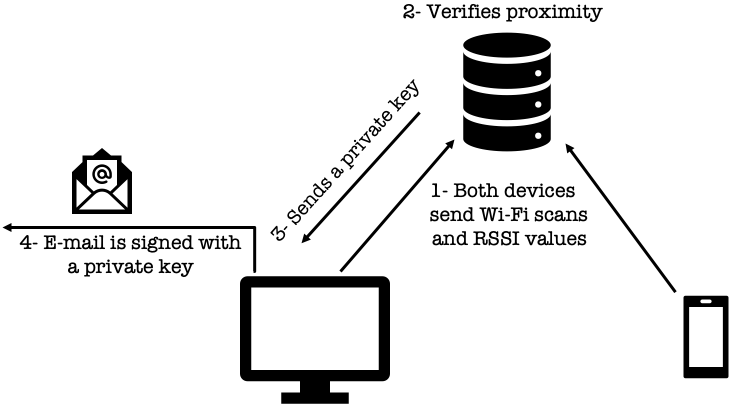
\includegraphics[width=\linewidth]{figures/figure_p3_1.png}
\caption{Overview}
\label{fig:1}
\end{figure}

\section{Experiment}
A smartphone application and a google chrome extension were designed to perform the proposed scheme. The applications reply to a request from the validation entity and scan all three access points. In the experimental setup, three access points were utilized at different positions in the user's environment. The three access points' exact standings were measured and located manually on the experiment site as a preliminary step. Moreover, x and y coordinates of seven different actual points were manually located within a room. A Wi- Fi-enabled device was placed at each point, then collected 20 RSSI values from each access point. \subsection{Position accuracy In this}  experiment, the collected RSSI values were plugged into equation (2) to find the estimated x and y coordinates of each the seven different points. Find the different between each actual point and its estimated x and y coordinate were estimated using (3). shows the estimated positions and the different between the actual and estimated points after utilizing the first RSSI value that the Wi-Fi-enabled device collected. shows the estimated x and y coordinate and the difference between the actual and estimated points after utilizing the average of 60 RSSI values. shows the estimated x and y coordinate and the difference between the actual and estimated points after utilizing the maximum of 60 RSSI values. FIRST RSSI VALUE RESULTS Actual points Estimated points Difference (2 , 17) (4.2 , 14.3) 3.6 ft (3 , 2) (1.3 , 7.7) 5.9 ft ( 4.5 , 9 ) (4.3 , 9.3) 0.3 ft ( 5 , 14 ) (4.1 , 12.3) 1.96 ft ( 6 , 2 ) (10.7 , -1) 5.6 ft ( 7 , 2 ) (-0.1 , 7.4) 8.9 ft ( 8 , 17 ) (6.4 , 9) 7.2 ft AVERAGE OF 60 RSSI VALUES RESULTS Actual points Estimated points Difference (2 , 17) (5.2 , 15.4) 3.6 ft (3 , 2) (1.4 , 7.5) 5.6 ft ( 4.5 , 9 ) (3.9 , 9.9) 0.98 ft ( 5 , 14 ) (4 , 12.6) 1.6 ft ( 6 , 2 ) (7 , 2.4) 0.98 ft ( 7 , 2 ) (3.2 , 4.5) 4.6 ft ( 8 , 17 ) (10.5 , 15) 2.6 ft 161 MAXIMUM OF 60 RSSI VALUES RESULTS Actual points Estimated points Difference (2 , 17) (4.2 , 14.3) 3.6 ft (3 , 2) (1.5 , 7.3) 5.6 ft ( 4.5 , 9 ) (3.3 , 10) 1.6 ft ( 5 , 14 ) (3.8 , 12.5) 1.97 ft ( 6 , 2 ) (5.3 , 4) 1.97 ft ( 7 , 2 ) (1.3 , 6.6) 7.5 ft ( 8 , 17 ) (4.6 , 9.9) 6.88 ft \subsection{Performance Measurement The validation performance}  rate of the proposed scheme was examined by utilizing every RSSI value to estimate the distance between two Wi-Fi-enabled devices; if the distance between the two device is 2 m or less validation is granted; otherwise, validation is denied. Then the results were run through a machine learning algorithm to generate a confusion matrix, . After that, the proposed scheme's validation success rate was computed using equation (4). As a result, the proposed scheme provided a 95.63\% validation success rate. TP + TN N × 100 (4) PERFORMANCE MEASUREMENT Actual N=1260 Positive Negative True 660 32 False 23 545

\begin{table}[H]
\caption{(x −x1)2 + (y −y1)2 = d2}
\label{tab:i}
\centering
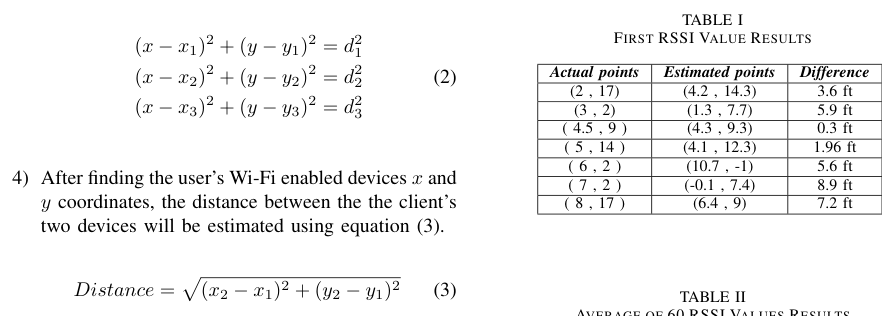
\includegraphics[width=\linewidth]{artifacts/tables/table_p3_1.png}
\end{table}

\begin{table}[H]
\caption{AVERAGE OF 60 RSSI VALUES RESULTS}
\label{tab:ii}
\centering
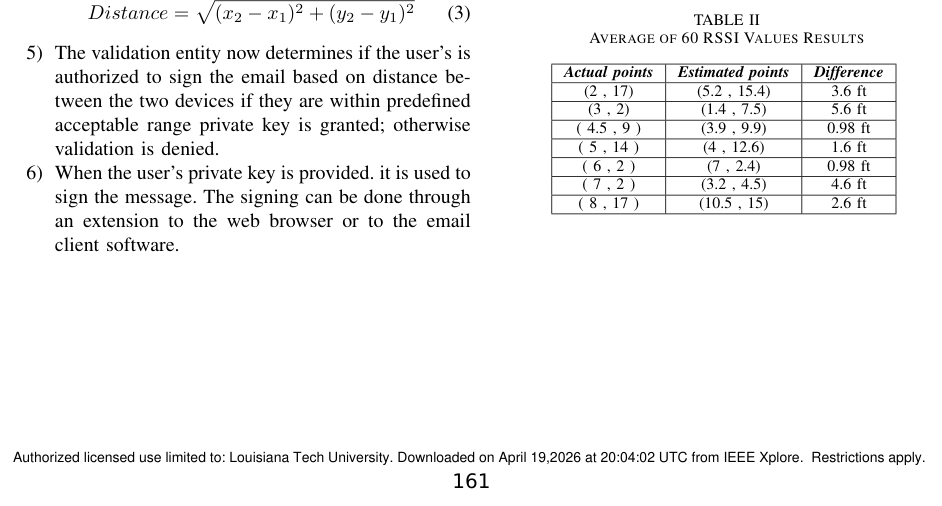
\includegraphics[width=\linewidth]{artifacts/tables/table_p3_2.png}
\end{table}

\begin{table}[H]
\caption{MAXIMUM OF 60 RSSI VALUES RESULTS}
\label{tab:iii}
\centering
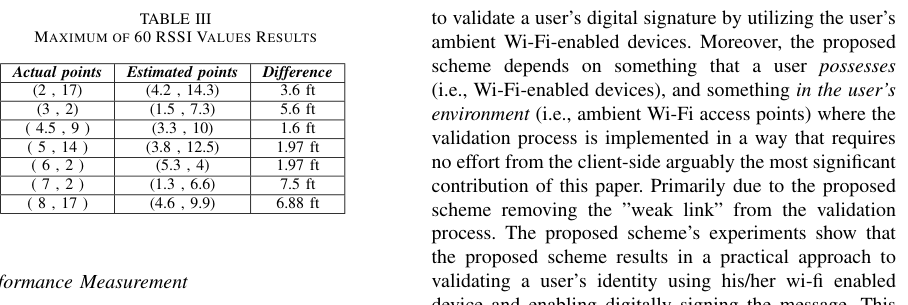
\includegraphics[width=\linewidth]{artifacts/tables/table_p4_1.png}
\end{table}

\begin{table}[H]
\caption{Systems for Video Technology, 18(4):549–553, 2008.}
\label{tab:iv}
\centering
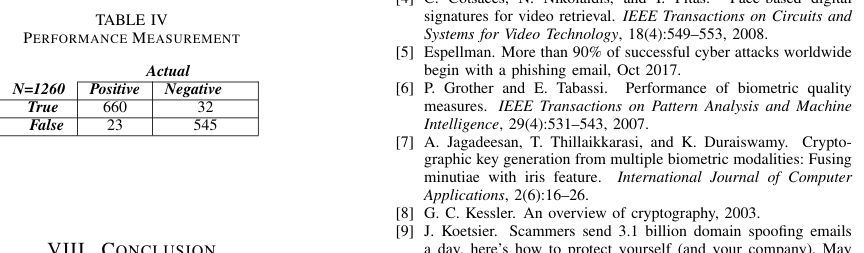
\includegraphics[width=\linewidth]{artifacts/tables/table_p4_2.png}
\end{table}

\begin{figure}[H]
\centering
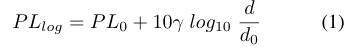
\includegraphics[width=0.72\linewidth]{artifacts/equations/equation_p3_1.png}
\end{figure}

\begin{figure}[H]
\centering
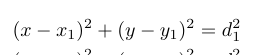
\includegraphics[width=0.72\linewidth]{artifacts/equations/equation_p3_2.png}
\end{figure}

\begin{figure}[H]
\centering
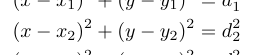
\includegraphics[width=0.72\linewidth]{artifacts/equations/equation_p3_3.png}
\end{figure}

\begin{figure}[H]
\centering
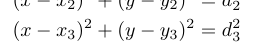
\includegraphics[width=0.72\linewidth]{artifacts/equations/equation_p3_4.png}
\end{figure}

\begin{figure}[H]
\centering
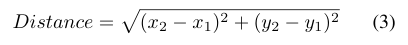
\includegraphics[width=0.72\linewidth]{artifacts/equations/equation_p3_5.png}
\end{figure}

\section{Conclusion}
A digital signature is a scheme for verifying the authenticity of digital messages, emails, or documents. A digital signature provides the recipient of the message to trust the authenticity of the received message that is coming from the said sender and that the message was not altered in transit. Digital signatures, like handwritten signatures, are unique to each signer. A digital signature uses Public Key Infrastructure (PKI). PKI requires the sender to generate two keys. One key is public, and the other key is private. For example, when a signer electronically signs of the received messages. This paper proposes a scheme to validate a user's digital signature by utilizing the user's scheme depends on something that a user possesses (i.e., Wi-Fi-enabled devices), and something in the user's environment (i.e., ambient Wi-Fi access points) where the validation process is implemented in a way that requires no effort from the client-side arguably the most significant contribution of this paper. Primarily due to the proposed scheme removing the "weak link" from the validation process. The proposed scheme's experiments show that the proposed scheme results in a practical approach to validating a user's identity using his/her wi-fienabled device and enabling digitally signing the message. This is done by utilizing the user's ambient Wi-Fi-enabled devices based on the distance between the two devices if they are within a predefined acceptable range the private key is provided and the message is signed automatically; otherwise, validation is denied. The proposed scheme is an efficient method with a validation accuracy of 95.63\%.

\begin{figure}[H]
\centering
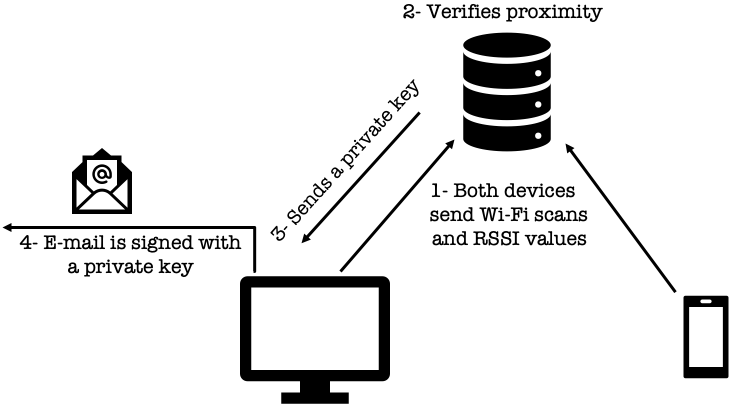
\includegraphics[width=\linewidth]{figures/figure_p3_1.png}
\caption{Extracted figure 1}
\label{fig:extracted1}
\end{figure}
\begin{figure}[H]
\centering
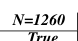
\includegraphics[width=0.72\linewidth]{artifacts/equations/equation_p4_1.png}
\end{figure}
\bibliographystyle{ACM-Reference-Format}
\bibliography{references}
\end{document}
